We examine the performance loss of pruned networks by introducing signal collapse - a phenomenon we observe for the first time, where one-shot pruning progressively reduces activation variance across layers, ultimately impairing the network’s ability to distinguish between inputs. In this section, we formally define signal collapse, explain its mechanisms, and demonstrate its impact on network performance. Finally, we introduce REFLOW, a method to mitigate signal collapse and restore the performance of one-shot pruned networks.
\subsection{Notation and Setup}

Consider a pre-trained neural network \( f(\theta) \), parameterized by \(\theta \in \mathbb{R}^d\). For a given layer \(\ell \in \{1, \dots, L\}\), let the input to layer \(\ell\) be denoted as \(\mathbf{H}_{\ell-1}\). The pre-BatchNorm (pre-BN) activation at layer \(\ell\) is defined as:
\begin{equation}
    \mathbf{X}_\ell = f(\mathbf{H}_{\ell-1}; \theta_\ell),
    \label{eq:pre_bn_signal_formal}
\end{equation}
where \(\theta_\ell\) represents the parameters of layer \(\ell\).

Batch Normalization (BN) normalizes the pre-BN activation \(\mathbf{X}_\ell\) across the batch as follows:
\begin{equation}
    \mathbf{Z}_\ell(n) = 
    \frac{\mathbf{X}_\ell(n) - \mu_\ell}
    {\sqrt{\mathrm{Var}_\ell^{\text{(Orig)}}(\mathbf{X}_\ell) + \epsilon}} \cdot \gamma_\ell + \beta_\ell,
    \label{eq:bn_transform}
\end{equation}
where \(n\) is the index of the batch dimension, \(\mu_\ell\) and \(\mathrm{Var}_\ell^{\text{(Orig)}}(\mathbf{X}_\ell)\) are the running mean and variance of the BN layer, \(\gamma_\ell\) and \(\beta_\ell\) are fixed affine parameters, and \(\epsilon > 0\) is a small constant for numerical stability.


\noindent \textbf{Defining Signal Collapse.}
\emph{Signal collapse} occurs in a pruned network if the variance of the activations reduces significantly in deeper layers compared to the original, unpruned network. Formally, let \(\mathrm{Var}_\ell^{(\text{Pruned})}\) and \(\mathrm{Var}_\ell^{(\text{Orig})}\) denote the variances of activations at layer \(\ell\) in the pruned and original networks, respectively. Signal collapse occurs if:
\begin{equation}
    \lim_{\ell \to L} 
    \frac{\mathrm{Var}_\ell^{(\text{Pruned})}}{\mathrm{Var}_\ell^{(\text{Orig})}}
    \;\to\; 0,
    \label{eq:signal_collapse_definition}
\end{equation}
where \(L\) is the total number of layers.

When the variance ratio approaches zero in deeper layers, the activations become nearly constant, resulting in a loss of distinction between inputs, causing uniform predictions.

\subsection{Why Pruning Causes Signal Collapse}
\label{subsec:mechanisms_signal_collapse}

Signal collapse arises due to two reasons explored below:

\paragraph{A) Activation variance reduces due to weight pruning}.

Pruning zeroes out weights based on a selection criterion, typically removing those with lower scores under the assumption that they contribute less to the network's performance. Formally, for layer \(\ell\), pruning modifies the weights \(\theta_\ell\) to \(\theta_\ell'\), where weights are set to zero if their score \(z_{i}\) falls below a threshold \(\tau\):
\begin{equation}
    W_{\ell,i}' = 
    \begin{cases}
        W_{\ell,i}, & \text{if } z_{i} > \tau \\
        0, & \text{otherwise}
    \end{cases},
    \label{eq:weight_pruning_general}
\end{equation}
where \(z_{i}\) represents the pruning score (e.g., magnitude, impact (loss) based heuristic, as discussed in Section \ref{sec:relatedwork}) for weight \(W_{\ell,i}\), and \(\tau\) is the pruning threshold determined by the desired sparsity level \(\kappa\).

To calculate the variance of the pre-BN activation after pruning, consider the activation in its pruned state:\begin{equation}
\mathbf{X}_\ell' = \sum_{i \in \mathcal{S}} W_{\ell,i}' H_{\ell-1,i},
\end{equation}
where \(\mathcal{S}\) is the set of non-pruned weights. Assuming that the activations \( H_{\ell-1,i} \) are independent and have a zero mean, the covariance terms between different \( H_{\ell-1,i} \) and \( H_{\ell-1,j} \) (for \( i \neq j \)) vanish. Therefore, the variance of \(\mathbf{X}_\ell'\) simplifies to:
\begin{equation}
    \mathrm{Var}_\ell^{\text{(Pruned)}}(\mathbf{X}_\ell') = \sum_{i \in \mathcal{S}} W_{\ell,i}'^2 \cdot \mathrm{Var}(H_{\ell-1,i}),
    \label{eq:pruned_variance}
\end{equation}

This leverages the property that the variance of a sum of independent random variables is the sum of their variances, and the scaling property \(\mathrm{Var}(aX) = a^2 \mathrm{Var}(X)\) for a constant \(a\).

Given that at high sparsity many weights are removed, especially those with lower scores, the sum in Equation~\ref{eq:pruned_variance} diminishes, leading to:
\begin{equation}
    \mathrm{Var}_\ell^{\text{(Pruned)}}(\mathbf{X}_\ell') \ll \mathrm{Var}_\ell^{\text{(Orig)}}(\mathbf{X}_\ell).
    \label{eq:variance_reduction}
\end{equation}
% This reduced variance is a direct consequence of pruning, as the removal of numerous low-scoring weights diminishes the diversity and scale of activations generated by each layer.

\paragraph{B) Over-Normalization due to BN mismatch}

As shown above, after one-shot pruning, pre-BN activations \(\mathbf{X}_\ell'\) have a lower variance, denoted as \(\mathrm{Var}_\ell^{\text{(Pruned)}}(\mathbf{X}_\ell')\). However, BN layers retain the original running statistics \((\mu_\ell, \mathrm{Var}_\ell^{\text{(Orig)}}(\mathbf{X}_\ell))\) computed prior to pruning. Consequently, the BN transformation for pruned activations is:
\begin{equation}
    \mathbf{Z}_\ell'(n) = 
    \frac{\mathbf{X}_\ell'(n) - \mu_\ell}
    {\sqrt{\mathrm{Var}_\ell^{\text{(Orig)}}(\mathbf{X}_\ell) + \epsilon}} \cdot \gamma_\ell + \beta_\ell.
    \label{eq:pruned_bn_variance}
\end{equation}
Here, both subtracting the mean \(\mu_\ell\) and adding  \(\beta_\ell\) do not affect the variance of $\mathbf{Z}_\ell'$, only the scaling factor \(\frac{\gamma_\ell}{\sqrt{\mathrm{Var}_\ell^{\text{(Orig)}}(\mathbf{X}_\ell) + \epsilon}}\) influences the variance of \(\mathbf{Z}_\ell'\).

Applying the property that \(\mathrm{Var}(aX) = a^2 \mathrm{Var}(X)\) for a constant \(a\), the variance of the post-BN activation becomes:
\begin{equation}
    \mathrm{Var}_\ell^{\text{(Pruned)}}(\mathbf{Z}_\ell') = \left( \frac{\gamma_\ell}{\sqrt{\mathrm{Var}_\ell^{\text{(Orig)}}(\mathbf{X}_\ell) + \epsilon}} \right)^2 \cdot \mathrm{Var}_\ell^{\text{(Pruned)}}(\mathbf{X}_\ell').
    \label{eq:var_z_pruned}
\end{equation}
Similarly, the variance of the original (unpruned) post-BN activation is:
\begin{equation}
    \mathrm{Var}_\ell^{\text{(Orig)}}(\mathbf{Z}_\ell) = \left( \frac{\gamma_\ell}{\sqrt{\mathrm{Var}_\ell^{\text{(Orig)}}(\mathbf{X}_\ell) + \epsilon}} \right)^2 \cdot \mathrm{Var}_\ell^{\text{(Orig)}}(\mathbf{X}_\ell).
    \label{eq:var_z_orig}
\end{equation}

Taking the ratio of the pruned to original post-BN variances:
\begin{equation}
    \frac{\mathrm{Var}_\ell^{\text{(Pruned)}}(\mathbf{Z}_\ell')}{\mathrm{Var}_\ell^{\text{(Orig)}}(\mathbf{Z}_\ell)} = \frac{\mathrm{Var}_\ell^{\text{(Pruned)}}(\mathbf{X}_\ell')}{\mathrm{Var}_\ell^{\text{(Orig)}}(\mathbf{X}_\ell)}.
    \label{eq:variance_ratio}
\end{equation}
Given that \(\mathrm{Var}_\ell^{\text{(Pruned)}}(\mathbf{X}_\ell') \ll \mathrm{Var}_\ell^{\text{(Orig)}}(\mathbf{X}_\ell)\) as established in Equation~\ref{eq:variance_reduction}, it follows that:
\begin{equation}
\mathrm{Var}_\ell^{\text{(Pruned)}}(\mathbf{Z}_\ell') \ll \mathrm{Var}_\ell^{\text{(Orig)}}(\mathbf{Z}_\ell).\label{eq:Z_diff}
\end{equation}
Thus, \textbf{Over-Normalization} causes post-BN activations to cluster closely around their mean, reducing their variance. 

\subsection{Cumulative Reduction in Activation Variance and Signal Collapse Across Layers}

Signal collapse arises because of the reduction in activation variance which \emph{cumulatively compounds} across deeper layers in the network. In this subsection, we analyze how this progressive decline emerges when considering post-BN outputs.

\noindent
\textbf{Scaling Factor \(\eta_\ell\).}
For each layer \(\ell\), define the \emph{variance scaling factor} \(\eta_\ell\) as:
\begin{equation}
    \eta_\ell 
    \;=\; 
    \frac{\mathrm{Var}_\ell^{\text{(Pruned)}}\!\bigl(\mathbf{Z}_\ell'\bigr)}
         {\mathrm{Var}_\ell^{\text{(Orig)}}\!\bigl(\mathbf{Z}_\ell\bigr)}
    \;<\; 1,
    \label{eq:scaling_factor}
\end{equation}
where \(\kappa \in [0,1]\) is the fraction of weights pruned. As \(\kappa \to 1\), more weights are removed, which generally makes \(\eta_\ell\) smaller via Equations \ref{eq:pruned_variance} and \ref{eq:Z_diff}.

\noindent
\textbf{Propagation of Variance Reduction.}
Because the \emph{input} to layer \(\ell+1\) is the \emph{post-BN} output of layer \(\ell\) (\(\mathbf{H}_{\ell+1} = \mathbf{Z}_\ell\)), the pruned input \(\mathbf{H}_{\ell+1}'\) is \(\mathbf{Z}_\ell'\). Consequently, any variance reduction at layer \(\ell\) affects layer \(\ell+1\), causing variance to shrink \emph{layer by layer} in the pruned network.

\noindent
\textbf{Cumulative Variance Scaling.}
Recursively applying Equation~\ref{eq:scaling_factor} across \(L\) layers, the cumulative variance scaling at the final layer $L$ becomes:
\begin{equation}
    \mathrm{Var}_L^{\text{(Pruned)}}\!\bigl(\mathbf{Z}_L'\bigr)
    \;=\;
    \Bigl(\,\prod_{\ell=1}^L \eta_\ell\Bigr)
    \,\mathrm{Var}_L^{\text{(Orig)}}\!\bigl(\mathbf{Z}_L\bigr).
    \label{eq:cumulative_variance}
\end{equation}
As an example consider the following. 
By assuming a modest constant per-layer scaling factor of \(\eta_\ell = 0.9\) across \(L = 25\) layers, the cumulative variance scaling becomes:
\begin{equation}
    \prod_{\ell=1}^{25} 0.9 = 0.9^{25} \approx 0.072.
    \label{eq:example_cumulative_variance}
\end{equation}


In practice, \(\eta_\ell\) varies across layers due to differences in sparsity distribution across layers, but the overall trend remains consistent: variance reduces as activations propagate through the pruned network. As \(\ell\) approaches \(L\), with increasing sparsity  \(\kappa\), 
\begin{equation}
    \;\;\lim_{\kappa \to 1}\;
    \mathrm{Var}_L^{\text{(Pruned)}}\bigl(\mathbf{Z}_L'\bigr)
    \;=\;
    \Bigl(\prod_{\ell=1}^L \eta_\ell\Bigr)\,
    \mathrm{Var}_L^{\text{(Orig)}}\!\bigl(\mathbf{Z}_L\bigr)
    \;\;\xrightarrow{}\;\;
    0,
    \label{eq:variance_approaching_zero}
\end{equation}
Consequently, the variance of the activations in the final layers approaches zero (see Figure~\ref{fig:variance_ratios}). 

\noindent
\textbf{Insight.}
Given that \(\mathrm{Var}_L^{\text{(Pruned)}}(\mathbf{Z}_L') \to 0\), the post-BN outputs converge to their mean (constant) value:
\begin{equation}
    \lim_{\mathrm{Var}(\mathbf{Z}_L') \to 0} 
    \;\mathbf{Z}_L'(n) 
    \;=\; 
    \mathrm{Mean}(\mathbf{Z}_L'(n))
    \label{eq:constant_activation}
\end{equation}
This implies that for any two distinct inputs \(\mathbf{x}_1\) and \(\mathbf{x}_2\),
$\mathbf{Z}_L'(\mathbf{x}_1) \approx \mathbf{Z}_L'(\mathbf{x}_2)$. We refer to this as \textit{signal collapse} (see Figure~\ref{fig:prediction_collapse}) and the network is incapable of distinguishing between inputs, thereby making it ineffective for downstream tasks, such as classification.





We empirically validate signal collapse using two \textbf{global scalar metrics} after each BN layer \(\ell\). These metrics summarize the behavior of normalized activations \(\mathbf{Z}_\ell\),


\begin{align}
    \mathrm{Mean}_\ell &= \frac{1}{|\mathbf{Z}_\ell|} \sum_{x \in \mathbf{Z}_\ell} x, \\
    \mathrm{Var}_\ell &= \frac{1}{|\mathbf{Z}_\ell|} \sum_{x \in \mathbf{Z}_\ell} \left( x - \mathrm{Mean}_\ell \right)^2.
\end{align}
where \(|\mathbf{Z}_\ell|\) denotes the total number of elements in the tensor \(\mathbf{Z}_\ell\). Figure~\ref{fig:variance_ratios} illustrates the signal variance ratio \(\frac{\mathrm{Var}_\ell^{\text{(Pruned)}}}{\mathrm{Var}_\ell^{\text{(Orig)}}}\) across layers at different sparsity levels \(\kappa\). The ratio progressively drops with increasing sparsity, remaining near 1 for 40\% sparsity, but drops below 0.1 after Layer~22 in 90\% sparsity, resulting in signal collapse.%, significantly compromising the network's ability to differentiate between inputs.


Figure~\ref{fig:prediction_collapse} demonstrates signal collapse in ResNet-20 on CIFAR-10. The unpruned model distributes predictions evenly across all classes in the test set. In contrast, at 90\% sparsity, the pruned network collapses, with over 99.4\% of inputs mapped to a single class. This behavior aligns with our analysis shown in Equation~\ref{eq:constant_activation}, leading to nearly identical representations for different inputs ($\mathbf{Z}'_L(\mathbf{x}_1) \approx \mathbf{Z}'_L(\mathbf{x}_2)$).


\begin{figure}[h]
\centering
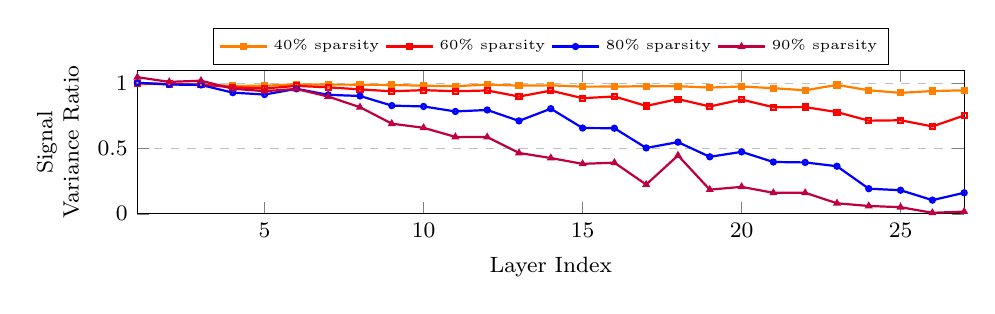
\begin{tikzpicture}
\begin{axis}[
    width=10.5cm,
    height=0.15\textwidth,
    scale only axis,
    xlabel={Layer Index},
    ylabel={Signal \\Variance Ratio},
    ylabel style={align=center},
    xmin=1, xmax=27,
    ymin=0, ymax=1.1,
    xtick={5,10,15,20,25},
    ymajorgrids=true,
    grid style=dashed,
    legend style={
        at={(0.5,+1.3)},
        anchor=north,
        font=\tiny,
        cells={anchor=west},
        inner sep=2pt,
        legend columns=4,
    },
    tick label style={font=\footnotesize},
    label style={font=\footnotesize},
    legend cell align=left,
    cycle list name=color list
]
% 40% sparsity
\addplot[color=orange, mark=square*, mark size=0.9pt, solid, thick] coordinates {
    (1,0.9982) (2,0.9968) (3,0.9934) (4,0.9820) (5,0.9844) (6,0.9947)
    (7,0.9928) (8,0.9922) (9,0.9898) (10,0.9843) (11,0.9805) (12,0.9928)
    (13,0.9851) (14,0.9870) (15,0.9771) (16,0.9775) (17,0.9806) (18,0.9806)
    (19,0.9700) (20,0.9784) (21,0.9651) (22,0.9490) (23,0.9904) (24,0.9490)
    (25,0.9293) (26,0.9433) (27,0.9487)
};

% 60% sparsity
\addplot[color=red, mark=square, mark size=0.9pt, solid, thick] coordinates {
    (1,1.0035) (2,0.9968) (3,0.9921) (4,0.9729) (5,0.9626) (6,0.9830) 
    (7,0.9717) (8,0.9561) (9,0.9413) (10,0.9502) (11,0.9416) (12,0.9476) 
    (13,0.9010) (14,0.9464) (15,0.8883) (16,0.9015) (17,0.8289) (18,0.8813) 
    (19,0.8248) (20,0.8777) (21,0.8190) (22,0.8200) (23,0.7814) (24,0.7156) 
    (25,0.7188) (26,0.6714) (27,0.7553)
};


% 80% sparsity
\addplot[color=blue, mark=o, mark size=0.9pt, solid, thick] coordinates {
    (1,1.0071) (2,0.9936) (3,0.9898) (4,0.9310) (5,0.9164) (6,0.9603) 
    (7,0.9142) (8,0.9054) (9,0.8313) (10,0.8248) (11,0.7865) (12,0.7979) 
    (13,0.7139) (14,0.8078) (15,0.6590) (16,0.6577) (17,0.5062) (18,0.5508) 
    (19,0.4380) (20,0.4762) (21,0.3983) (22,0.3949) (23,0.3657) (24,0.1931) 
    (25,0.1815) (26,0.1053) (27,0.1616)
};


% 90% sparsity
\addplot[color=purple, mark=triangle, mark size=0.9pt, solid, thick] coordinates {
    (1,1.0497) (2,1.0136) (3,1.0227) (4,0.9611) (5,0.9423) (6,0.9593)
    (7,0.9009) (8,0.8193) (9,0.6927) (10,0.6609) (11,0.5910) (12,0.5896)
    (13,0.4677) (14,0.4287) (15,0.3839) (16,0.3930) (17,0.2250) (18,0.4487)
    (19,0.1859) (20,0.2073) (21,0.1615) (22,0.1616) (23,0.0810) (24,0.0605)
    (25,0.0511) (26,0.0081) (27,0.0171)
};
\addlegendentry{40\% sparsity}
\addlegendentry{60\% sparsity}
\addlegendentry{80\% sparsity}
\addlegendentry{90\% sparsity}
\end{axis}
\end{tikzpicture}
\caption{Layer-wise signal variance ratios $
    \frac{\mathrm{Var}^{\text{(Pruned)}}}{\mathrm{Var}^{\text{(Orig)}}},
    \label{eq:variance_ratio}$ in pruned MobileNet (on ImageNet). Higher sparsity leads to severe signal collapse in deeper layers.}\label{fig:variance_ratios}
\end{figure}


\begin{figure}[t]
\centering
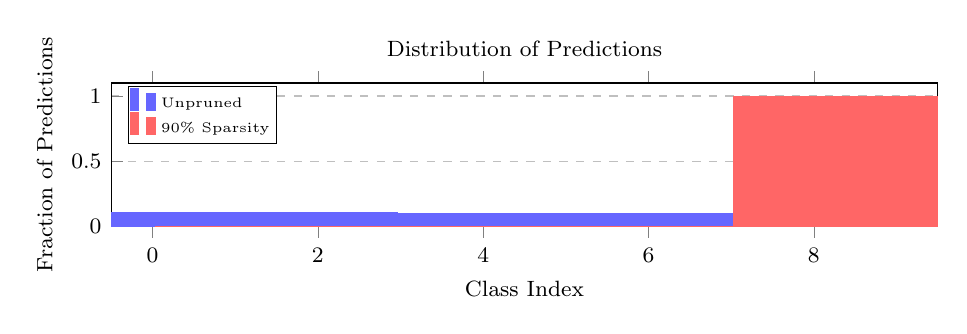
\begin{tikzpicture}
% Distribution Plot
\begin{axis}[
    width=10.5cm,
    height=0.15\textwidth,
    scale only axis,
    xlabel={Class Index},
    ylabel={Fraction of Predictions},
    xmin=-0.5, xmax=9.5,
    ymin=0, ymax=1.1,
    xtick={0,2,4,6,8},
    ymajorgrids=true,
    grid style=dashed,
    legend style={
        at={(0.02,0.98)},
        anchor=north west,
        font=\tiny,
        cells={anchor=west},
        inner sep=0.5pt,
        legend columns=1,
        scale=0.65,
        row sep=-2pt,
    },
    tick label style={font=\footnotesize},
    label style={font=\footnotesize},
    title={\footnotesize Distribution of Predictions},
    ybar,
    bar width=3,
]
% Original distribution
\addplot[blue!60, fill=blue!60] coordinates {
    (0,0.099600) (1,0.101300) (2,0.100100) (3,0.101500) (4,0.099300)
    (5,0.098900) (6,0.100600) (7,0.099900) (8,0.098700) (9,0.100100)
};
\addlegendentry{Unpruned}

% Updated 90% Pruned distribution
\addplot[red!60, fill=red!60] coordinates {
    (0,0.000000) (1,0.000000) (2,0.000500) (3,0.000000) (4,0.000000)
    (5,0.000000) (6,0.000000) (7,0.994800) (8,0.000000) (9,0.004700)
};
\addlegendentry{90\% Sparsity}
\end{axis}
\end{tikzpicture}
\caption{Distribution of predictions made by ResNet-20 on CIFAR-10. The unpruned model predicts uniformly across classes, discriminating between inputs, while the pruned model maps most inputs to a single class.}
\label{fig:prediction_collapse}
\end{figure}



\subsection{Hessian-Based Updates Mitigate but Do Not Fully Solve Signal Collapse}

Building on our earlier findings that Hessian-based updates are essential to recovering accuracy after pruning, we examine the effect of these updates on signal collapse. Specifically, we analyze how these updates influence the variance of activations across network layers.

\paragraph{Impact of Hessian-Based Updates on Signal Variance}

Figure~\ref{fig:variance_updates} presents the layer-wise signal variance ratios \(\frac{\mathrm{Var}_\ell^{\text{(Pruned)}}}{\mathrm{Var}_\ell^{\text{(Orig)}}}\) for three pruning methods: \textbf{CHITA-S} (selection-only), \textbf{MP-S} (Magnitude Pruning selection-only), and \textbf{CHITA-U} (selection with Hessian-based updates). 

As presented in Section~\ref{sec:revisiting_weight_selection}, \textbf{CHITA-S} and \textbf{MP-S} make near similar pruning decisions, resulting in identical (overlapping) variance profiles. Both pruning methods undergo signal collapse, with variance ratios frequently below 1 across layers. In contrast, \textbf{CHITA-U} maintains higher variance ratios in most layers, indicating that Hessian-based updates may help mitigate signal collapse. However, a few layers deeper in the network still show reduced variance ratios. This suggests that while Hessian-based updates reduce the impact of signal collapse, they do not entirely prevent it.

\begin{figure}[h]
\centering
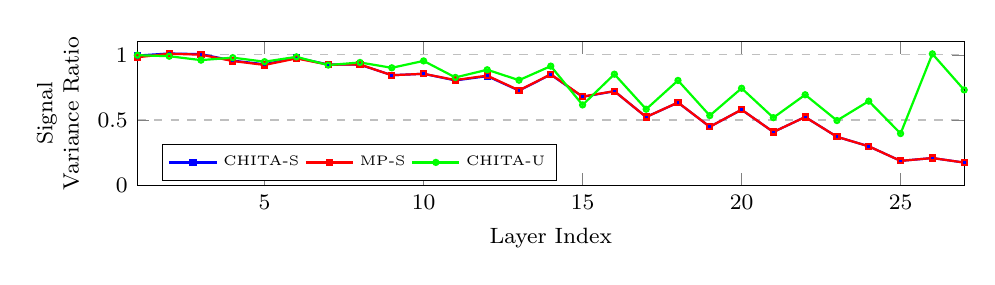
\begin{tikzpicture}
\begin{axis}[
    width=10.5cm,
    height=0.15\textwidth,
    scale only axis,
    xlabel={Layer Index},
    ylabel={Signal \\Variance Ratio},
    ylabel style={align=center},
    xmin=1, xmax=27,
    ymin=0, ymax=1.1,
    xtick={5,10,15,20,25},
    ymajorgrids=true,
    grid style=dashed,
    legend pos=south west,
    legend style={
        font=\tiny,
        cells={anchor=west},
        inner sep=2pt,
        legend columns=3,
    },
    tick label style={font=\footnotesize},
    label style={font=\footnotesize},
    legend cell align=left,
    cycle list name=color list
]
% CHITA-S
\addplot[color=blue, mark=square*, mark size=0.9pt, solid, thick] coordinates {
    (1,0.995) (2,1.011) (3,1.006) (4,0.956) (5,0.928) (6,0.978)
    (7,0.927) (8,0.925) (9,0.844) (10,0.855) (11,0.804) (12,0.837)
    (13,0.726) (14,0.849) (15,0.678) (16,0.721) (17,0.523) (18,0.634)
    (19,0.448) (20,0.579) (21,0.408) (22,0.523) (23,0.371) (24,0.298)
    (25,0.186) (26,0.208) (27,0.173)
};
% MP-S
\addplot[color=red, mark=square, mark size=0.9pt, solid, thick] coordinates {
    (1,0.982) (2,1.009) (3,1.002) (4,0.953) (5,0.923) (6,0.973)
    (7,0.925) (8,0.926) (9,0.844) (10,0.855) (11,0.807) (12,0.841)
    (13,0.728) (14,0.851) (15,0.680) (16,0.722) (17,0.523) (18,0.635)
    (19,0.448) (20,0.580) (21,0.408) (22,0.523) (23,0.371) (24,0.298)
    (25,0.186) (26,0.208) (27,0.173)
};
% CHITA-U
\addplot[color=green, mark=o, mark size=0.9pt, solid, thick] coordinates {
    (1,0.998) (2,0.990) (3,0.960) (4,0.979) (5,0.948) (6,0.985)
    (7,0.922) (8,0.942) (9,0.901) (10,0.954) (11,0.827) (12,0.886)
    (13,0.806) (14,0.914) (15,0.616) (16,0.852) (17,0.583) (18,0.804)
    (19,0.534) (20,0.744) (21,0.518) (22,0.694) (23,0.496) (24,0.645)
    (25,0.396) (26,1.008) (27,0.731)
};
\addlegendentry{CHITA-S}
\addlegendentry{MP-S}
\addlegendentry{CHITA-U}
\end{axis}
\end{tikzpicture}
\caption{Layer-wise signal variance ratios $\frac{\mathrm{Var}^{\text{(Pruned)}}}{\mathrm{Var}^{\text{(Baseline)}}}$ in 80\% sparse MobileNet on ImageNet. \textbf{CHITA-S} and \textbf{MP-S} show identical levels of signal collapse, while \textbf{CHITA-U} mitigates this collapse by Hessian-based updates.}\label{fig:variance_updates}
\end{figure}




\subsection{REFLOW: Restoring Signal Propagation to Mitigate Collapse}

\emph{Signal collapse} due to pruning stems from diminished activation variance. Hessian-based IP methods only partially mitigate signal collapse by updating the unpruned weights. These observations point to a more direct solution: if the core issue is the compounding mismatch between the pruned and original activation variances \(\frac{\mathrm{Var}_\ell^{\text{(Pruned)}}}{\mathrm{Var}_\ell^{\text{(Orig)}}} < 1\), resulting in signal collapse (Equation~\ref{eq:signal_collapse_definition}), then the running BN statistics can be calibrated to induce activation variance to mitigate signal collapse,  \emph{without} updating any unpruned (trainable) weights.


We propose \textbf{REFLOW} (\textbf{Re}storing \textbf{F}low of \textbf{Low}-variance signals), which updates only the BN running mean and variance after one-shot pruning. Specifically, rather than relying on the pre-pruning BN statistics $\bigl(\mu_\ell,\;\mathrm{Var}_\ell^{(\text{Orig})}\bigr)$, we collect a small calibration set $\mathcal{B}$ ($O(10)$ training batches) and pass it through the pruned network, and compute:
\begin{align}
\widehat{\mu}_\ell^{(\text{Pruned})}
  &= \frac{1}{|\mathcal{B}|} \sum_{n \in \mathcal{B}} \mathbf{X}_\ell'(n), \\
\widehat{\mathrm{Var}}_\ell^{(\text{Pruned})}(\mathbf{X}_\ell')
  &= \frac{1}{|\mathcal{B}|} \sum_{n \in \mathcal{B}}
    \Bigl(\mathbf{X}_\ell'(n) - \widehat{\mu}_\ell^{(\text{Pruned})}\Bigr)^2,
  \label{eq:reflow_calib}
\end{align}
where $\mathbf{X}_\ell'(n)$ are the pre-BN activations in the pruned model. We replace 
$\bigl(\mu_\ell,\;\mathrm{Var}_\ell^{(\text{Orig})}\bigr)$
with $\bigl(\widehat{\mu}_\ell^{(\text{Pruned})},\;\widehat{\mathrm{Var}}_\ell^{(\text{Pruned})}\bigr)$ in the BN layers, leaving $\gamma_\ell,\;\beta_\ell$ and all unpruned weights unchanged. The resulting post-BN activations become:
\begin{equation}
  \mathbf{Z}_\ell'^{(\text{REFLOW})}(n)
  \;=\;
  \frac{\mathbf{X}_\ell'(n) - \widehat{\mu}_\ell^{(\text{Pruned})}}
       {\sqrt{\widehat{\mathrm{Var}}_\ell^{(\text{Pruned})}(\mathbf{X}_\ell') + \epsilon}}
  \;\gamma_\ell \;+\; \beta_\ell.
  \label{eq:reflow_transform}
\end{equation}

\smallskip \noindent \textbf{Preserving Signal Variance}: REFLOW aligns each BN layer’s statistics with the \emph{true} statistics of the pruned pre-BN activations. This offsets the cumulative loss of variance that causes signal collapse. Figure~\ref{fig:reflow_effect}, shows recalibration at high sparsities restores the post-BN variance to the levels of the unpruned network. In doing so, REFLOW improves the network’s discriminative power by mitigating signal collapse without retraining or updating unpruned weights.




\begin{figure}[h]
\centering
\begin{tikzpicture}
\begin{groupplot}[
    group style={
        group size=2 by 1,
        horizontal sep=10pt,
        vertical sep=0pt
    },
    width=7.5cm,
    height=0.24\textwidth,
    xlabel={Layer Index},
    xmin=1,
    ymin=0, ymax=1.1,
    ymajorgrids=true,
    grid style=dashed,
    tick label style={font=\footnotesize},
    label style={font=\footnotesize},
    legend cell align=left
]

%------------------ RESNET-20 ------------------%
\nextgroupplot[
    xmax=21,
    xtick={1,5,10,15,20},
    ylabel={Signal \\ Variance Ratio},
    ylabel style={align=center},
    title={\footnotesize ResNet-20 (CIFAR-10)}
]
\addplot[color=red, mark=square, mark size=0.7pt, solid, thick] coordinates {
(1,1.0345) (2,0.8172) (3,0.9096) (4,0.8688) (5,0.9972) (6,1.0141) (7,0.6961) (8,0.8730) (9,0.7257) (10,0.9861) (11,0.6367) (12,0.5695) (13,0.5532) (14,0.5492) (15,0.5341) (16,0.5009) (17,0.7034) (18,0.4376) (19,0.2782) (20,0.3987) (21,0.2088)};

\addplot[color=blue, mark=o, mark size=0.7pt, solid, thick] coordinates {
(1,1.0045) (2,1.0033) (3,1.0071) (4,1.0047) (5,1.0007) (6,0.9972) (7,0.9942) (8,1.0043) (9,1.0030) (10,1.0049) (11,1.0036) (12,1.0056) (13,1.0025) (14,1.0055) (15,1.0020) (16,0.9995) (17,1.0086) (18,0.9994) (19,0.9895) (20,1.0033) (21,0.8669)};

%------------------ MOBILENET ------------------%
\nextgroupplot[
    xmax=27,
    xtick={1,5,10,15,20,25},
    ytick = \empty,
    legend style={
        at={(0.03,0.03)},
        anchor=south west,
        font=\tiny,
        cells={anchor=west},
    },
    title={\scriptsize MobileNet (ImageNet)}
]
\addplot[color=red, mark=square, mark size=0.7pt, solid, thick] coordinates {
    (1,0.982) (2,1.009) (3,1.002) (4,0.953) (5,0.923) (6,0.973)
    (7,0.925) (8,0.926) (9,0.844) (10,0.855) (11,0.807) (12,0.841)
    (13,0.728) (14,0.851) (15,0.680) (16,0.722) (17,0.523) (18,0.635)
    (19,0.448) (20,0.580) (21,0.408) (22,0.523) (23,0.371) (24,0.298)
    (25,0.186) (26,0.208) (27,0.173)
};
\addlegendentry{MP}

\addplot[color=blue, mark=o, mark size=0.7pt, solid, thick] coordinates {
(1,0.9857) (2,1.0085) (3,1.0091) (4,1.0037) (5,1.0035) (6,0.9124) (7,1.0100) (8,0.9989) (9,0.9944) (10,1.0039) (11,1.0013) (12,0.9932) (13,0.9930) (14,1.0024) (15,1.0000) (16,1.0021) (17,1.0000) (18,1.0021) (19,0.9981) (20,1.0000) (21,1.0016) (22,0.9972) (23,0.9983) (24,0.9904) (25,0.9976) (26,0.9318) (27,0.9710)};
\addlegendentry{MP + REFLOW}

\end{groupplot}
\end{tikzpicture}

\caption{Layer-wise signal variance ratios in pruned networks under magnitude pruning at 80\% sparsity, before and after applying REFLOW.}
\label{fig:reflow_effect}
\end{figure}

